% -----------------------------------------------
% Template for ISMIR Papers
% 2017 version, based on previous ISMIR templates

% Requirements :
% * 6+n page length maximum
% * 4MB maximum file size
% * Copyright note must appear in the bottom left corner of first page
% * Clearer statement about citing own work in anonymized submission
% (see conference website for additional details)
% -----------------------------------------------

\documentclass{article}
\usepackage{ismir,amsmath,url}
\usepackage[nocompress]{cite}
\usepackage{graphicx}
\usepackage{color}
\usepackage{array}
\usepackage{tabularx}
\usepackage{arydshln}
\usepackage{lipsum}
\usepackage{multirow}
%\usepackage[table, xcdraw]{xcolor}
\usepackage{rotating}

\newcommand{\carl}[1]{\textcolor{blue}{#1}}
\newcommand{\izzy}[1]{\textcolor{red}{#1}}
\newcommand{\maciek}[1]{\textcolor{green}{#1}}
\newcommand{\jason}[1]{\textcolor{orange}{#1}}




%\renewcommand\note[1]{}


%\newcommand\myworries[1]{\textcolor{red}{#1}}
% Title.
% ------
%\title{Paper Template For ISMIR \conferenceyear}
\title{PLAYER IDENTIFICATION FOR TRADITIONAL IRISH FLUTE RECORDINGS}

% Note: Please do NOT use \thanks or a \footnote in any of the author markup

% Single address
% To use with only one author or several with the same address

%\oneauthor
%{Islah Ali-MacLachlan, Maciej Tomczak, Carl Southall, Jason Hockman}
%{DMT Lab, Birmingham City University \\ {\tt islah.ali-maclachlan, maciej.tomczak, carl.southall, jason.hockman} \\{\tt @bcu.ac.uk}}

% Three addresses
% --------------
\threeauthors
  {First Author} {Affiliation1 \\ {\tt author1@ismir.edu}}
  {Second Author} {\bf Retain these fake authors in\\\bf submission to preserve the formatting}
  {Third Author} {Affiliation3 \\ {\tt author3@ismir.edu}}
% ---------------


\sloppy % please retain sloppy command for improved formatting

\begin{document}

%
\maketitle
%
\begin{abstract}

The abstract should be placed at the top left column and should contain about 150-200 words.

\lipsum[1-2]


\end{abstract}
%
\section{Introduction}\label{sec:introduction}


\sloppypar{Irish Traditional Music (ITM) has progressed from its roots of social dance music to become a medium for listening. Represented at several large-scale music festivals in Europe and the US, and over 1500 weekly 'sessions' where musicians can meet and share repertoire, the indigenous music of Ireland has a large, international audience \cite{vallely_companion_2011}. 

Playing of the wooden simple system flute  in ITM was historically linked predominantly to the west and northwest of Ireland. The Irish cultural revival has allowed the flute to play a wider role as an intrinsic part of the sound of ITM alongside tin whistles, accordions, and fiddles \cite{williams_irish_2010}. 

%\begin{figure}[h]
%\begin{center}
%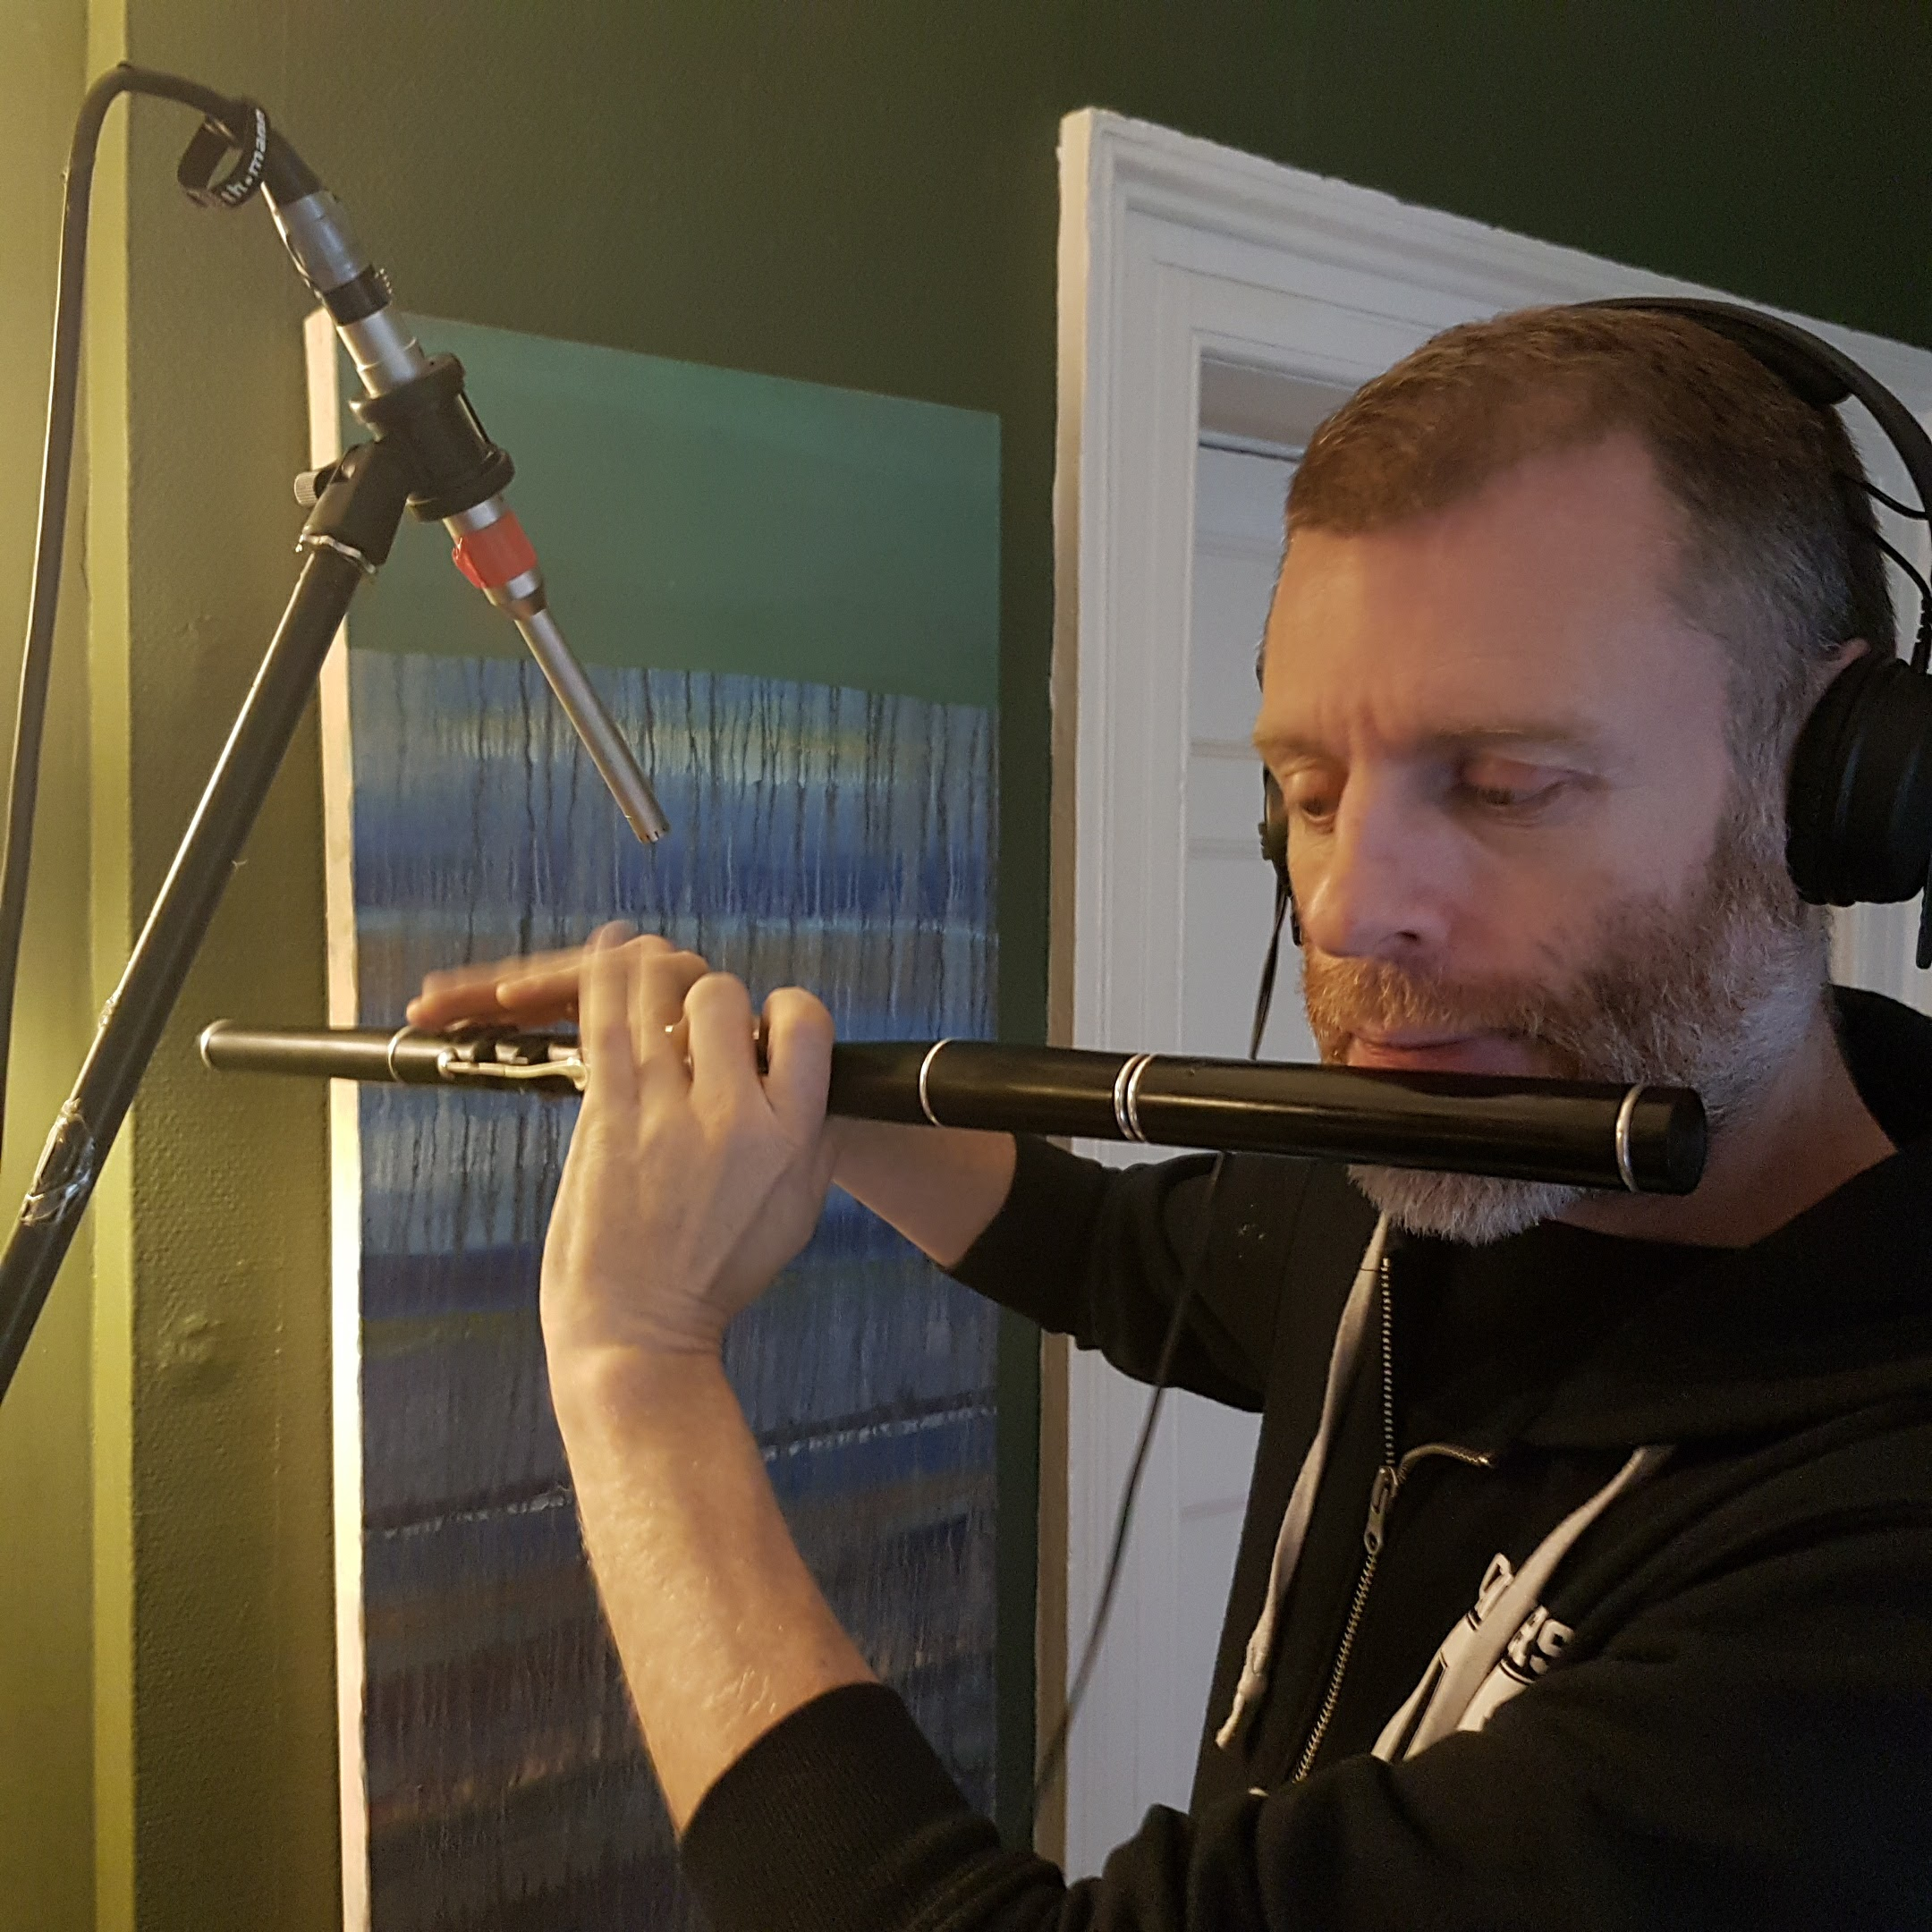
\includegraphics[width=0.45\textwidth]{figs/p4-1.jpg}
%\caption{Player with keyed blackwood simple system flute.}
%\label{fig:flute1}
%\end{center}
%\end{figure}

 Traditional flute players are individuated based on their use of techniques such as ornamentation, phrasing and articulation 
\cite{mccullough_style_1977,hast_music_2004, keegan_parameters_2010, larsen_essential_2003} alongside idiosyncratic timbral differences \cite{ali-maclachlan_quantifying_2013, widholm_silver_2001, ali-maclachlan_towards_2015}. Mastery is judged by creativity and technical ability within the stylistic bounds of traditional music and distinctive characteristics often develop organically as a player learns and refines their skills.  

In order to determine stylistic differences between players, we must first develop methods to detect these differences in audio signals. We evaluate recordings produced by six accomplished traditional flute players, all playing music from a predetermined corpus offering a range of typical modes and rhythms.

\subsection{Related work} \label{sec: Related Work}

 


Automatic music genre classification was initially introduced by Tzanetakis \& Cook \cite{tzanetakis_musical_2002} who proposed a framework for the development and analysis of features for music content analysis. As part of this work, mel-frequency cepstral coefficients (MFCC) features \cite{logan_mel_2000} were implemented due to their efficient representation of spectral data. Since then, several authors have proposed systems for genre and artist identification. 

Li and Ogihara \cite{li_music_2004} implemented a semi-supervised learning system with timbral features such as MFCC, spectral centroid, rolloff and flux as input alongside lyrical content.  Mandel \& Ellis \cite{mandel_song-level_2005} used support vector machines (SVM) to identify a single popular music performer from a group of 18 in the \emph{uspop2002} corpus \cite{berenzweig_large-scale_2004,ellis_d._uspop2002_2003}. Input features were segmented 20 band  MFCC extracted using the method described in \cite{pachet_improving_2004}. An important feature of this study was to explore and negate the 'album effect' \cite{kim_towards_2006,whitman_artist_2001} where songs from a single album are spectrally more similar than songs from different albums. 

State of the art identification techniques have been used as part of automatic music classification. Convolutional neural networks (CNN) have been used successfully with input features derived from spectrograms \cite{lee_unsupervised_2009} and MFCC representing timbre, tempo and key variations \cite{li_automatic_2010}. A CNN was trained to perform artist and genre recognition on the 'Million Song Dataset' \cite{bertin-mahieux_million_2011} using segments related to note onsets and feature vectors containing timbre and chroma components \cite{dieleman_audio-based_2011}. Lidy \& Schindler \cite{lidy_parallel_2016} used CNN to classify genre, mood and composer and achieved the highest results in MIREX 2016 using a 40-band Mel filter.

Costa et al \cite{costa_evaluation_2017} reinforced the effectiveness of CNN for music genre classification, performing analysis against SVM on three separate databases containing Western, Latin and African music. The CNN system compared favourably in a number of scenarios, particularly in the case of African music where the sources were largely field recordings. This method showed favourable results with multiple class types labelled country, function, ethnic group and instrumentation. Individual instrument classification is discussed in \cite{park_musical_2015} and as part of an ensemble in \cite{han_deep_2017}.

Studies in flute acoustics have found that individual players produce markedly different timbres while changes in material make very small spectral differences \cite{backus_effect_1964, coltman_effect_1971, widholm_silver_2001}. Previous methods of player detection in ITM have used signal processing methods \cite{ali-maclachlan_quantifying_2013, ali-maclachlan_towards_2015}. The use of probabilistic modelling, in particular CNN, is an important step in more accurate player identification. We propose a CNN system for identification of flute players in ITM in order to make use of their ability to efficiently process large datasets.

The remainder of this paper is structured as follows: Section \ref{sec:method}  details CNN and their implementation. In Section \ref{sec:evaluation} we discuss evaluation of.... Results of the studies into ... are presented in Section \ref{sec:results} and finally conclusions and further work are discussed in Section \ref{sec:conclusions}.

\begin{figure*}[t]
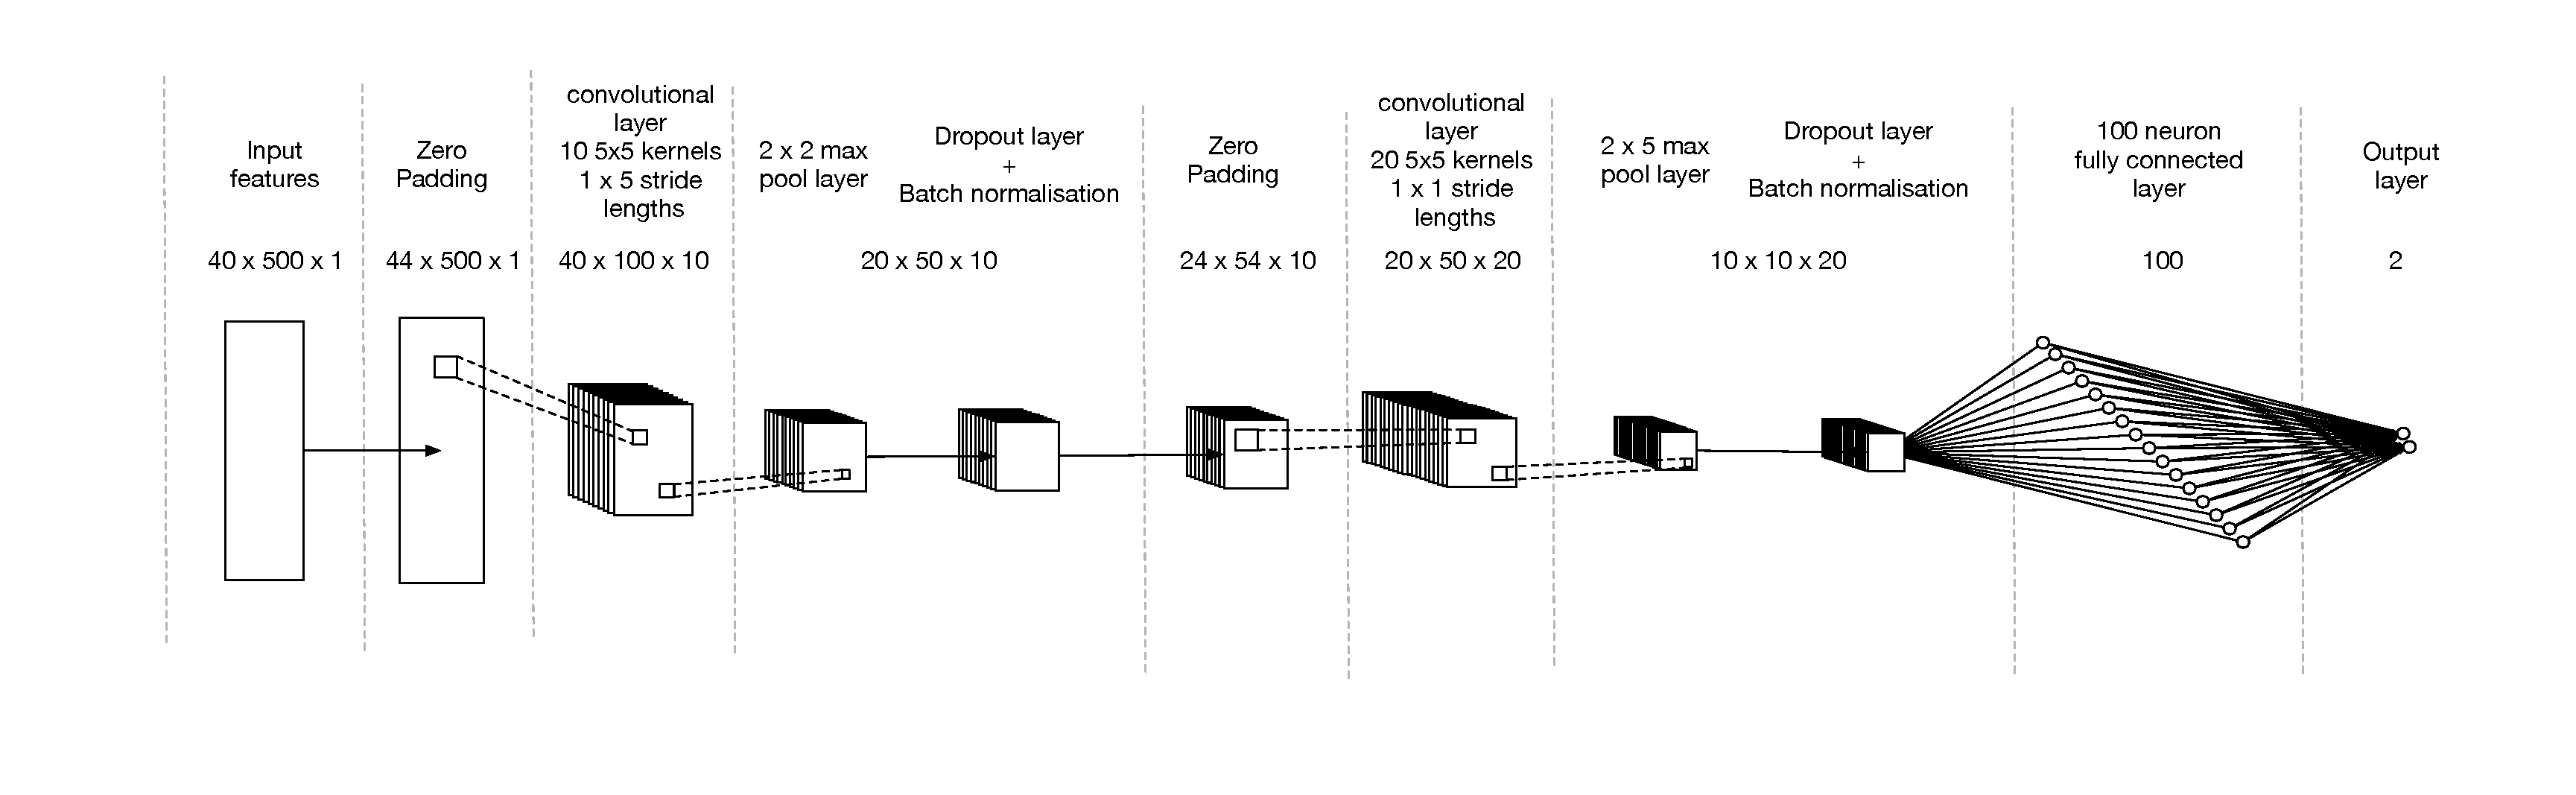
\includegraphics[width=1\textwidth]{figs/CNNDiagramPD}
\caption{Overview of the proposed implemented CNN system.}
\label{CNNDiagram}
\end{figure*}

\section{Method} \label{sec:method}

\izzy{Introductory paragraph}




\subsection{Convolutional neural networks (CNN)}
In order to capture the stylistic differences between each player we divide recordings into 5 second segments. We then extract timbral features as these are important in class distinction. Each player contributes distinct timbral features as part of their style. For that purpose we extract 40 MFCCs, excluding the first coefficient, to accommodate for differences in timbre over a range of played notes.%

%
CNNs enable larger input feature sizes to be used by first reducing the dimensionality of the features using a shared weighted kernel and pooling before they are input into a fully connected layer. This ability has enabled CNNs to achieve higher accuracies than recurrent neural networks in closed related fields including onset detection, beat detection and downbeat detection. REFEERENCES  An overview of the implemented CNN ADT systems with different input feature sizes is outlined in Figure... REF. All of the implement versions consist of two sets of convolutional, max pooling, dropout, and batch normalisation layers before a 100 neuron fully connected layer and a two neuron softmax output layer. The output $h$ of a two-dimensional convolutional layer with a rectified linear unit transfer function is calculated using:

\begin{equation}\label{eqn:conv}
 h^f_{ij}=r\Bigg(\sum_{l=0}^{L-1}\sum_{m=0}^{M-1} W^f_{ml}x_{(iu+l)(jv+m)}+b^f\Bigg)
\end{equation}

where $x$ is the input features, $W$ and $b$ are the shared weights and bias and $f$ is the feature map. $L$ and $M$ are the dimensions of the shared weight matrix and $I$ and $J$ are the output dimensions of that layer. $u$ and $v$ are the stride lengths and the equation for the rectifier linear unit transfer function $r$ is:

\begin{equation}\label{eqn:rect}
r(\phi)=max(0,\phi)
\end{equation}

Before the features $x$ are input into the network they are zero padded.

The output of the convolutional layer $h$ is then processed using a max pooling layer where the maximum of $a$ by $b$ sub-regions is taken. Dropouts are then performed on the output of the max pooling layer with a dropout probability of 0.25 and batch normalisation is implemented. \carl{IN DEPTH DETAIL ON BATCH NORM!}.

The output of the second batch normalisation $h_{bnL}$ layer is then input into a dense fully-connected layer ($Q=h_{bnL}$) Equation.{\ref{eqn:output} with a rectifier linear unit transfer function ($\sigma(\phi)=r(\phi)$) Equation.\ref{eqn:rect}. The output layer of the implemented CNNs is the same as the output layer of the SABRNN systems with the input to the layer being the output of the fully connected layer ($Q=h_fc$).


\subsection{Implementation}

\subsubsection{Input Features}



\subsubsection{Training Procedure}

The implemented models are trained using the Adam optimizer and a learning rate of 0.003.  Mini-batch gradient descent is used with batch sizes of 250. Training is stopped when a minimum of 50 iterations have commenced and the
validation set accuracy has not increased between iterations. The weights are initialized using a scaled uniform distribution \cite{DBLP:journals/corr/Sussillo14}
and biases are initialized to 0. Cross entropy is used as the loss function.


\section{Evaluation} \label{sec:evaluation}

\subsection{Dataset}\label{sec:dataset}
For these evaluations, we require a dataset that is representative of a range of respected players with individual stylistic traits. The dataset, containing 247 recordings of traditional 'tunes' played on solo flute, includes two discrete sections. The first section\footnote{recordings used in this section are available at: https://github.com/izzymaclachlan/datasets} comprises of 28 recordings by each of 6 experienced players (168 total) and the second section includes 79 released recordings of 9 professional players detailed in \cite{ali-maclachlan_islah_note_2016}. Only the first section was used in evaluation 1 (see Section \ref{sec:results}) whereas sections 1 and 2 were both used in evaluation 2.

The dataset is representative of the four most popular melodic styles, namely the reel, jig, hornpipe and polka \cite{hast_music_2004}. The structure of most traditional melodies in ITM can be attributed to two scales, D and G, and four classes defined by the ending note of the tune and given the solfa name Doh, Ray, Soh and Lah \cite{breathnach_folk_1996, o_canainn_traditional_1978}. 

The corpus of tunes shown in Table {\ref{tab:corpusTunes} was chosen to be representative of a typical player repertoire and to represent a range of scales and classes. 6 players played each tune twice without tempo restriction and twice in time with a click track played through headphones and set to represent a typical tempo according to \cite{breathnach_ceol_1963}. Players also recorded two other tunes picked from their own repertoire.

\begin{table}[]
\centering

\label{tab:corpusTunes}
\begin{tabular}{|l|c|c|c|c|}
\hline
\multicolumn{1}{|c|}{\textbf{No.}} & \textbf{Tune Title}& \textbf{Type} & \textbf{Scale} & \textbf{\begin{tabular}[c]{@{}c@{}}Ends\\ on\end{tabular}} \\ \hline
1&Maids of Mount Cisco                      & Reel          & G              & Ray                                                         \\ \hline
2&The Banshee                               & Reel          & G              & Soh                                                         \\ \hline
3&Cooley's Reel                             & Reel          & G              & Lah                                                         \\ \hline
4&Banish Misfortune                         & Jig           & G              & Doh                                                         \\ \hline
5&Morrison's Jig                            & Jig           & D              & Ray                                                         \\ \hline
6&The Home Ruler                            & Hornpipe      & D              & Doh                                                         \\ \hline
7&Players choice 1                            & ?      & ?              & ?                                                         \\ \hline
8&Players choice 2                            & ?      & ?              & ? \\ \hline
\end{tabular}
\caption{Corpus recorded by all players detailing tune type, scale and ending note. \carl{added numbers so correspond to results and wild tracks}}
\end{table}


\subsubsection{Recording} \label{sec:recording}
The recordings were collected as 16-bit/44.1kHz WAV files using a Thomann MM-1 measurement microphone connected to an Audient ID14 audio interface. The microphone was positioned above the middle of the flute in order to minimise wind noise. 
 



\subsection{Evaluation of methods}\label{sec:evalmeth}






\section{Results and Discussion}\label{sec:results}

\begin{figure}[h]
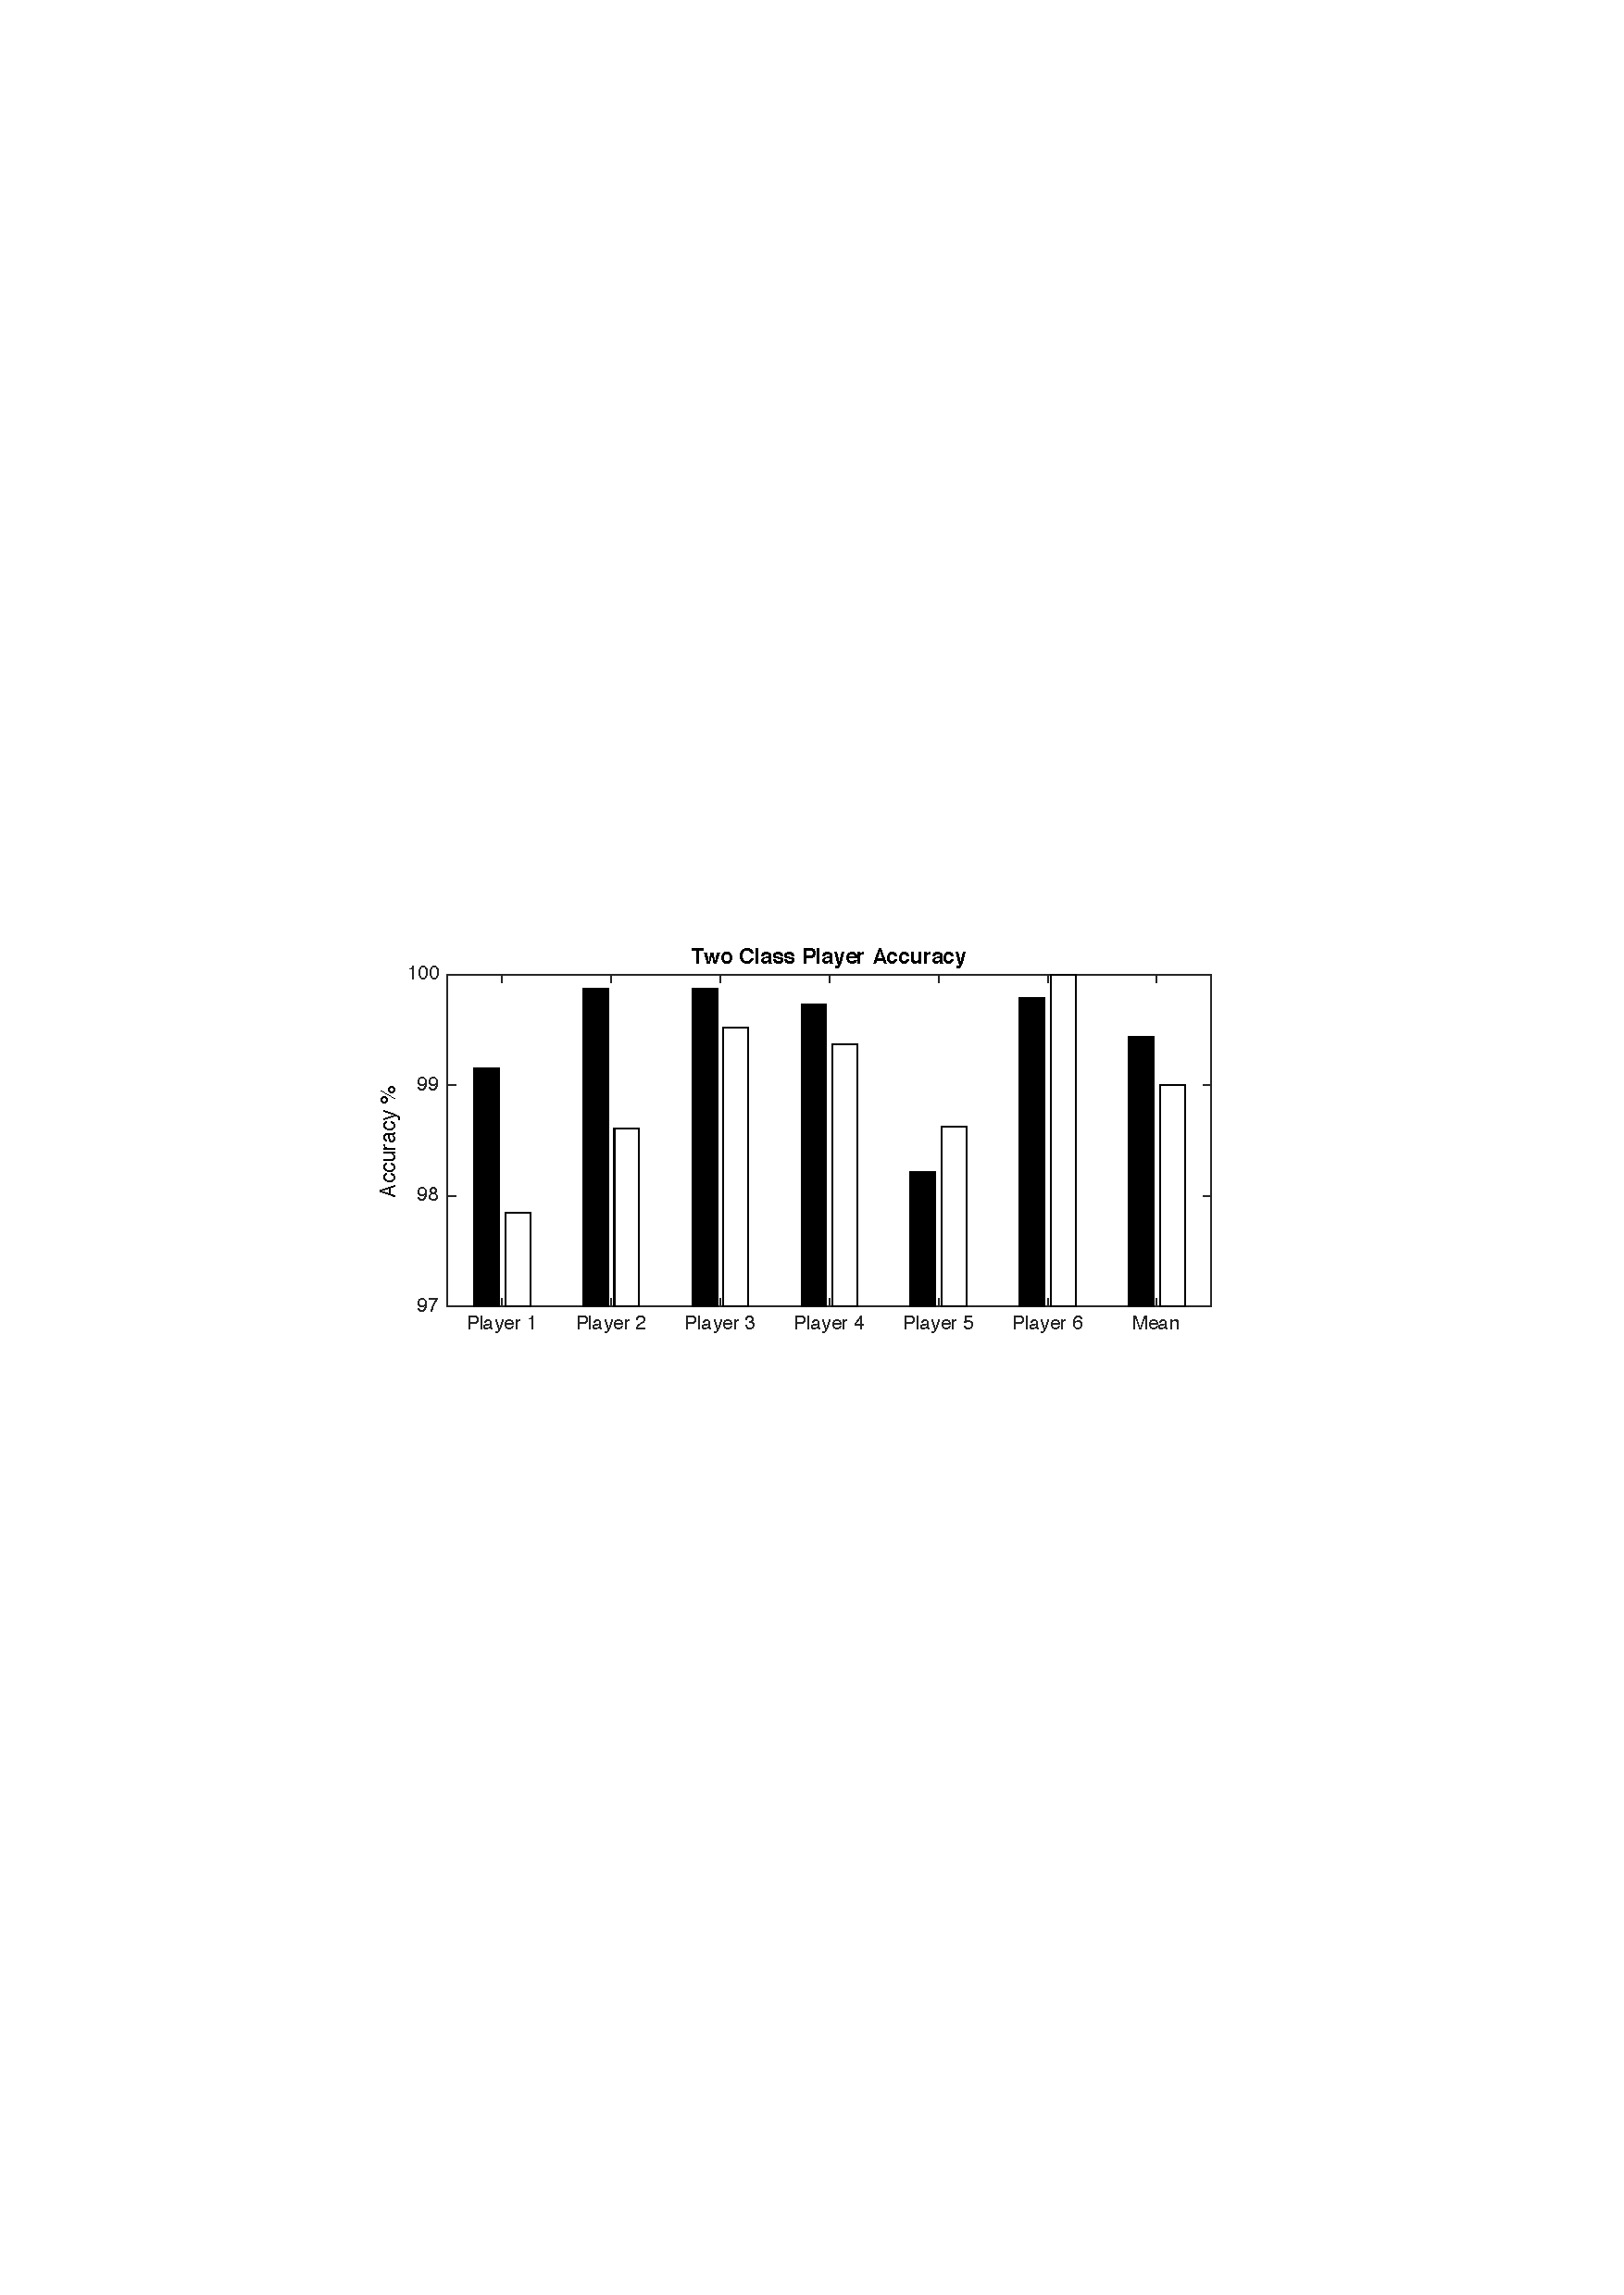
\includegraphics[width=0.5\textwidth]{figs/PlayerPDF}
\caption{Two class results per player and the mean across players.}
\label{PlayerGraph}
\end{figure}

\subsection{Two Class}

Figure \ref{PlayerGraph} presents the two class results for each player and the mean across players. As expected, a higher mean player accuracy is achieved in the 6 player evaluation than the 6 player and other evaluation. Player 4 achieves the lowest classification accuracy where as player 5 achieves the highest \carl{do we know why this is? Izzy? would be good discussion here if so...}.

A confusion matrix for the mean player results is presented in table \ref{2classconf}. For the 6 player evaluation the errors are roughly evenly distributed however, in the 6 player and other evaluation there is a larger number of the player tracks classified as other. \carl{again discuss why this is?}.

Table \ref{subgroups} presents the number of tracks that were correctly classified as the players tracks (upper left boxes in Table \ref{2classconf}) in each of the subgroups. \carl{again discuss what and why}.

\begin{table}[h!]
    
    \begin{minipage}{.5\linewidth}
      \centering

\begin{tabular}{cc|c|c|}

\cline{3-4}
\multicolumn{1}{l}{}                                          & \multicolumn{1}{l|}{} & \multicolumn{2}{c|}{\textbf{Pred}}                              \\ \cline{3-4} 
\multicolumn{1}{l}{}                                          & \multicolumn{1}{l|}{} & \textbf{P} & \textbf{O}  \\ \hline
\multicolumn{1}{|c|}{\multirow{2}{*}{\begin{turn}{90}\textbf{GT}\end{turn}}} & \textbf{P}            & 99.7     & 0.6            \\ \cline{2-4} 
\multicolumn{1}{|c|}{}                                        & \textbf{O}            & 0.3          & 99.4            \\ \hline
\end{tabular}
    \end{minipage}%across players
    \begin{minipage}{.5\linewidth}
      \centering
\begin{tabular}{cc|c|c|}

\cline{3-4}
\multicolumn{1}{l}{}                                          & \multicolumn{1}{l|}{} & \multicolumn{2}{c|}{\textbf{Pred}}                              \\ \cline{3-4} 
\multicolumn{1}{l}{}                                          & \multicolumn{1}{l|}{} & \textbf{P} & \textbf{O}  \\ \hline
\multicolumn{1}{|c|}{\multirow{2}{*}{\begin{turn}{90}\textbf{GT}\end{turn}}} & \textbf{P}            & 97.5    & 0.8            \\ \cline{2-4} 
\multicolumn{1}{|c|}{}                                        & \textbf{O}            & 2.5          & 99.2            \\ \hline
\end{tabular}
    \end{minipage} 
 \caption{Two class confusion matrices where pred is the predicted class, GT is the ground truth class, P is the player class and O the other class. 6 player evaluation is on the left and the 6 player and other evaluation is on the right.}
 \label{2classconf}   
\end{table}


\begin{table}[h!]

    \begin{minipage}{.5\linewidth}
      \centering
across players
\begin{tabular}{|c|c|c|}
\cline{2-3}
\multicolumn{1}{l|}{}&\textbf{1} & \textbf{2}  \\ \hline
\textbf{M}            & 99.7     & 100            \\ \cline{1-3} 
\textbf{N}            & 100          & 100            \\ \hline
\end{tabular}d Player
    \end{minipage}%
    \begin{minipage}{.5\linewidth}
      \centering
\begin{tabular}{|c|c|c|}
\cline{2-3}
\multicolumn{1}{l|}{}&\textbf{1} & \textbf{2}  \\ \hline
\textbf{M}            & 95.0   & 96.7            \\ \cline{1-3} 
\textbf{N}            & 97.3          & 98.8            \\ \hline
\end{tabular}across players
    \end{minipage} 
        \caption{Two class subgroup accuracies where M is metronome, N is no metronome, 1 is take 1 and 2 is take 2. 6 player evaluation is on the left and the 6 player and other evaluation is on the right.}
        \label{subgroups}
\end{table}
%
\begin{figure}[h]
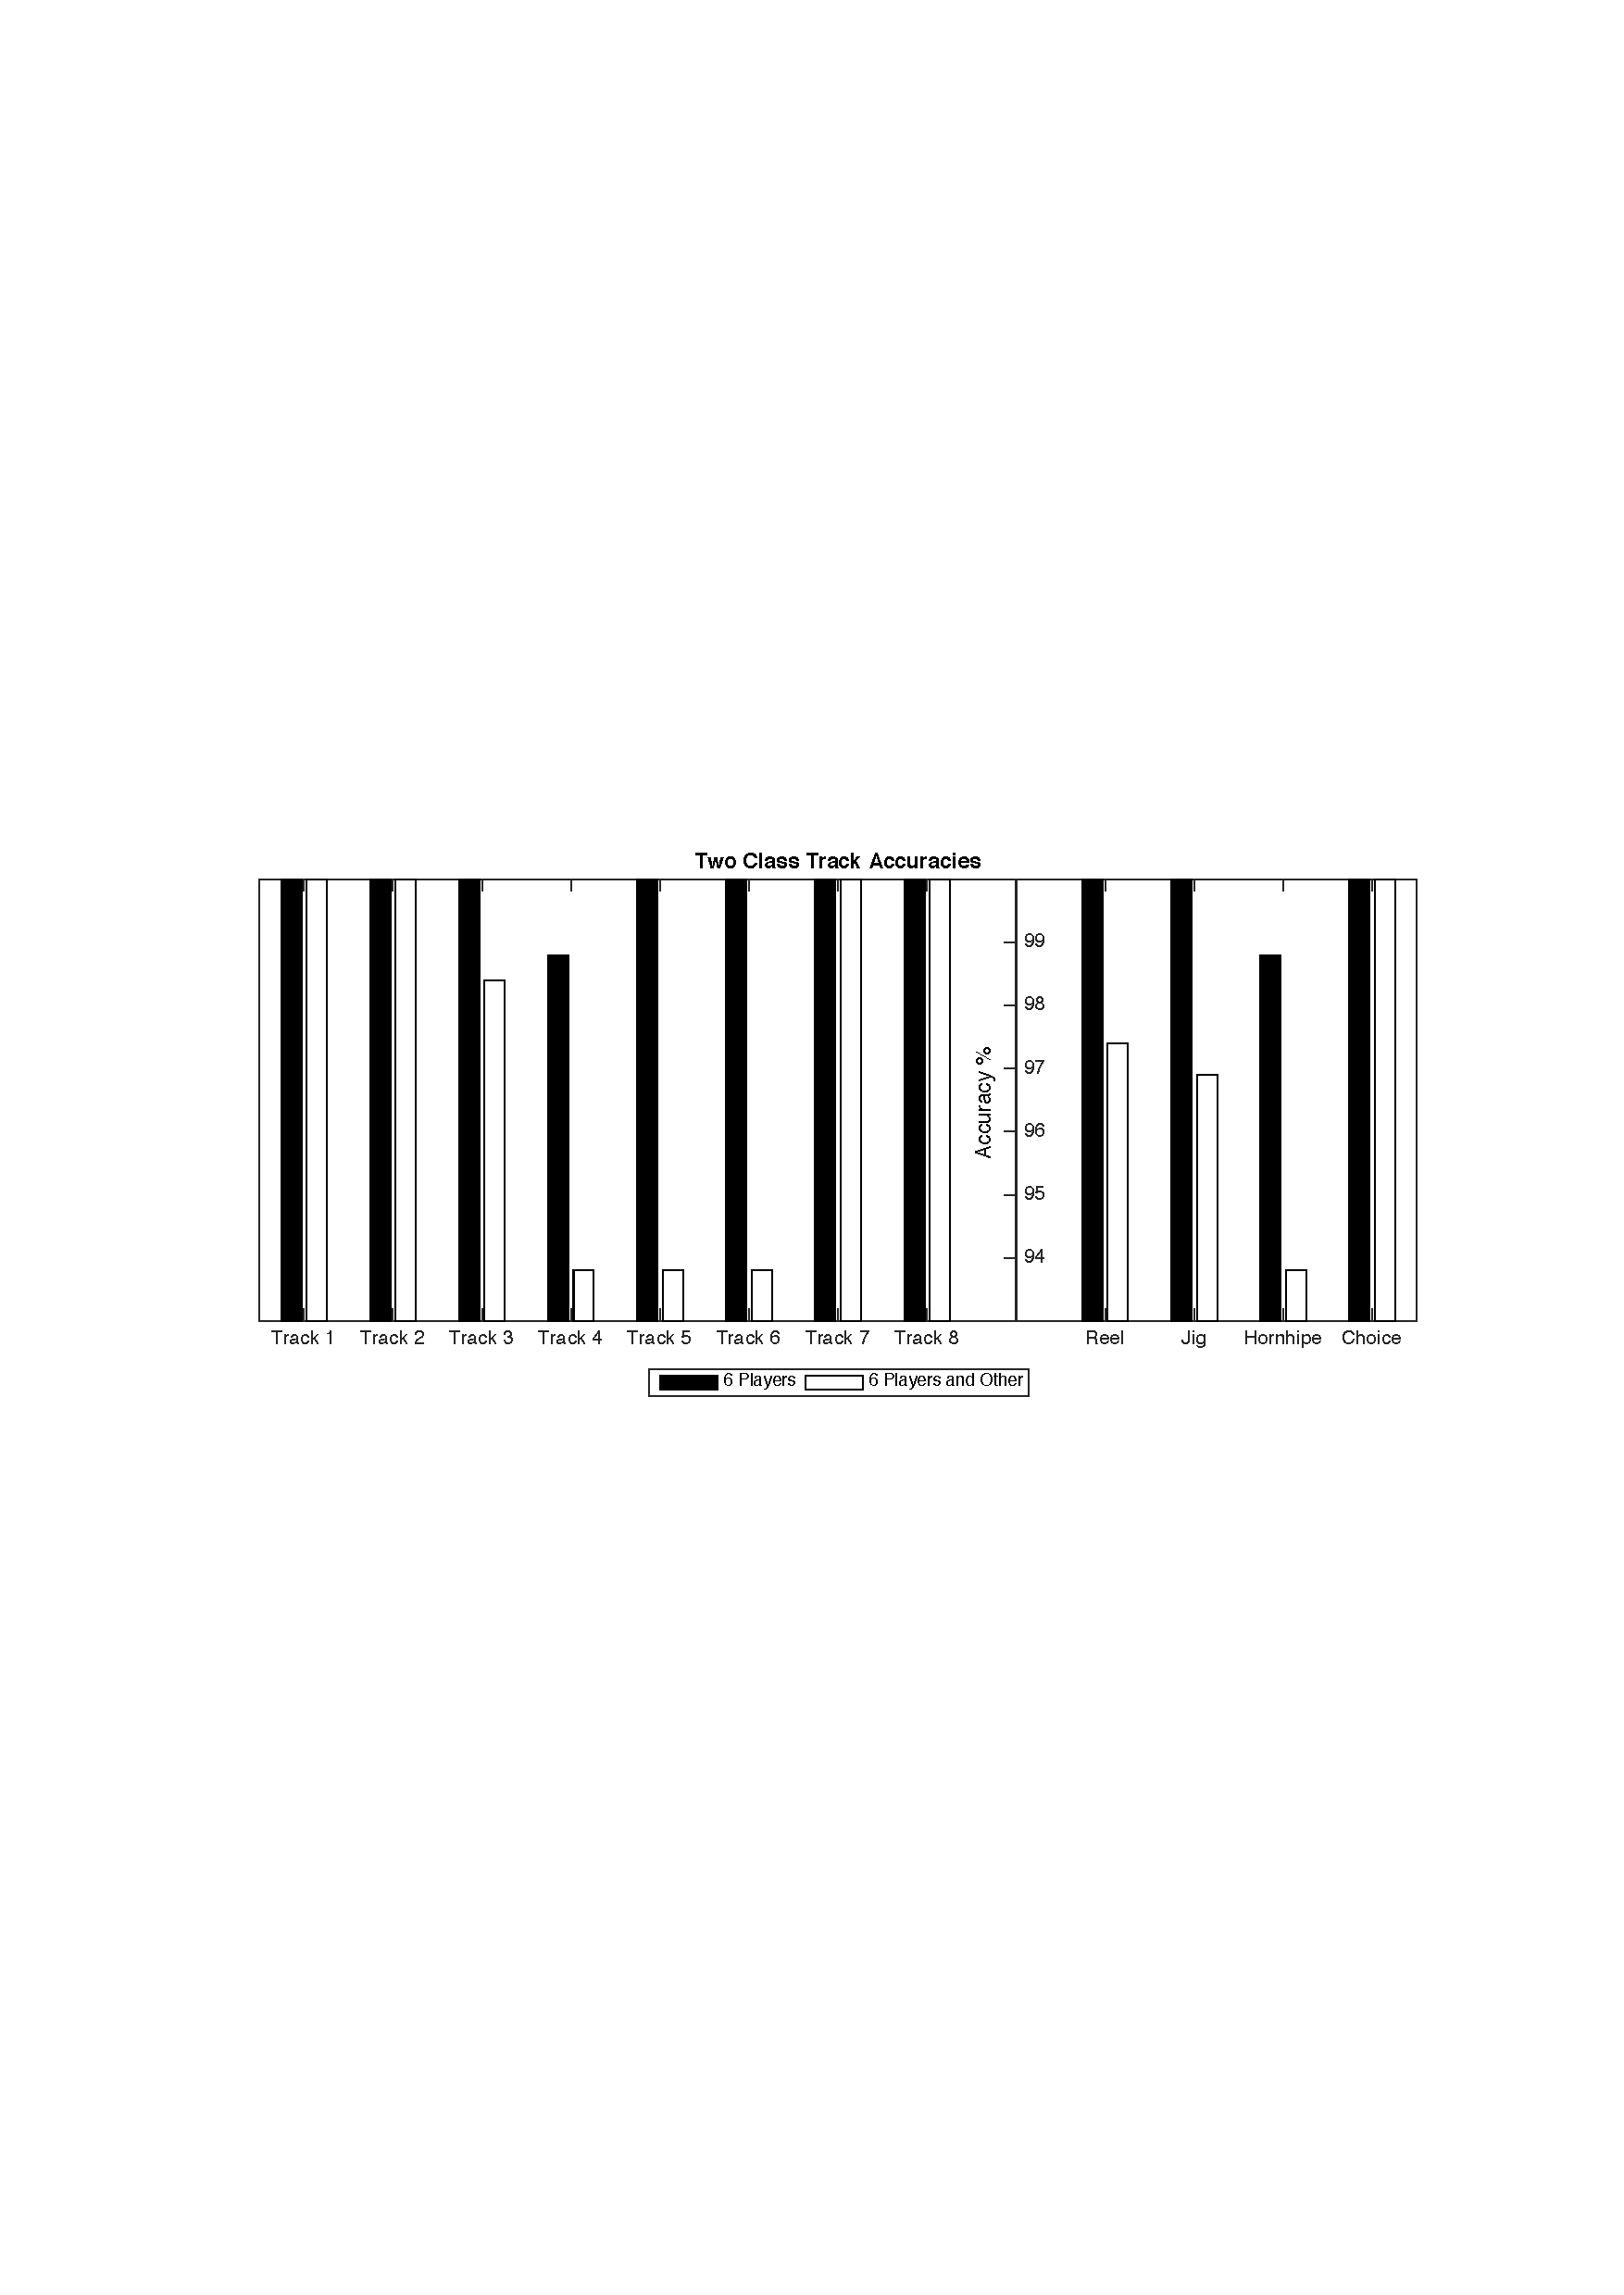
\includegraphics[width=0.5\textwidth]{figs/TrackPDF}
\caption{Two class results per track and the mean for the different track types.}
\label{TrackGraph}
\end{figure}

Figure \ref{TrackGraph} presents the percentage of the player tracks correctly classified as the players (same as Table \ref{subgroups}) for each of the tracks. Also presented are the mean accuracies for the track types. \carl{again what and why?}. 

\subsection{Individual Class}

\begin{table*}[h!]

    \begin{minipage}{.5\linewidth}
      \centering


\begin{tabular}{cc|c|c|c|c|c|c|}
\cline{3-8}
\multicolumn{1}{l}{}                                     & \multicolumn{1}{l|}{} & \multicolumn{6}{c|}{\textbf{Prediction}}                              \\ \cline{3-8} 
\multicolumn{1}{l}{}                                          & \multicolumn{1}{l|}{} & \textbf{1} & \textbf{2} & \textbf{3} & \textbf{4} & \textbf{5} & \textbf{6} \\ \hline
\multicolumn{1}{|c|}{\multirow{6}{*}{\begin{turn}{90}\textbf{Ground Truth}\end{turn}}} & \textbf{1}            & 98.8     & 0          & 0          & 0          & 0          & 0          \\ \cline{2-8} 
\multicolumn{1}{|c|}{}                                        & \textbf{2}            & 0          & 
100    & 0          & 0          & 0          & 0          \\ \cline{2-8} 
\multicolumn{1}{|c|}{}                                        & \textbf{3}            & 0          & 0          & 100     & 0          & 0.6     & 0          \\ \cline{2-8} 
\multicolumn{1}{|c|}{}                                        & \textbf{4}            & 0          & 0          & 0          & 100     & 0.9     & 0          \\ \cline{2-8} 
\multicolumn{1}{|c|}{}                                        & \textbf{5}            & 1.2     & 0          & 0          & 0          & 98.5     & 0          \\ \cline{2-8} 
\multicolumn{1}{|c|}{}                                   & \textbf{6}            & 0          & 0          & 0          & 0          & 0          & 100     \\ \hline
\end{tabular}
    \end{minipage}%
    \begin{minipage}{.5\linewidth}
      \centering
\begin{tabular}{cc|c|c|c|c|c|c|c|}
\cline{3-9}
\multicolumn{1}{l}{}                                          & \multicolumn{1}{l|}{} & \multicolumn{7}{c|}{\textbf{Prediction}}                                               \\ \cline{3-9}
\multicolumn{1}{l}{}                                          & \multicolumn{1}{l|}{} & \textbf{1} & \textbf{2} & \textbf{3} & \textbf{4} & \textbf{5} & \textbf{6} & \textbf{O} \\ \hline
\multicolumn{1}{|c|}{\multirow{7}{*}{\begin{turn}{90}\textbf{Ground Truth}\end{turn}}} & \textbf{1}            & 96     & 0.8     & 0          & 1.7           
     & 0          & 0          & 0              \\ \cline{2-9} 
\multicolumn{1}{|c|}{}                                        & \textbf{2}            & 0.7     & 97.8     & 0          & 0          & 0          & 0          & 0.8         \\ \cline{2-9} 
\multicolumn{1}{|c|}{}                                        & \textbf{3}            & 0.8      & 0          & 97.9     & 0          & 0.6     & 0          & 3.4        \\ \cline{2-9} 
\multicolumn{1}{|c|}{}                                        & \textbf{4}            & 0          & 0          & 0          & 98.3     & 0          & 0          & 2.3         \\ \cline{2-9} 
\multicolumn{1}{|c|}{}                                        & \textbf{5}            & 2.5      & 0          & 2.1     & 0          & 98.8     & 0          & 0.4         \\ \cline{2-9} 
\multicolumn{1}{|c|}{}                                        & \textbf{6}            & 0          & 0          & 0          & 0          & 0          & 100     & 1.3         \\ \cline{2-9} 
\multicolumn{1}{|c|}{}                                        & \textbf{O}        & 0          & 1.4     & 0          & 0          & 0.6     & 0          & 91.8         \\ \hline
\end{tabular}%

    \end{minipage} 
    \caption{Individual class confusion matrices. 6 player evaluation is on the left and the 6 player and other evaluation is on the right.}
      \label{indconfs}  
\end{table*}

Table \ref{indconfs} presents confusion matrices for the individual classification evaluation. The mean accuracies achieved are 99.6\% and 96.6\% for the 6 players and 6 players and others evaluations respectively. \carl{again what and why?}.



/carl{Notes: 6 player + 6 player and other need better names!}

\section{Conclusions and Future Work} \label{sec:conclusions}
%In this paper we present a note, cut and strike detection method for traditional Irish flute recordings. Our chosen approach to this problem is that of inter-onset segment classification using feed-forward neural networks. To evaluate the effectiveness of this approach we first conducted an evaluation of various onset detection algorithms on our dataset with the hope of using this method as a first step in the feature extraction. 
%
%When using ground truth onset annotations, we achieved 86\%, 70\% and 74\% accuracies for note, cut and strike classification respectively. When using detected onsets to train the neural network we achieved poor classification results. We then performed an analysis of the detected onsets and the context in which they appear to establish both the degree of the errors and the musical patterns in which they occur.
%
%In the future we intend to work on improving the automated detection of note events. We will also develop note and ornament classification methods with additional features and other neural network architectures (e.g., recurrent neural networks, networks with long short-term memory) in order to capture trends that appear in time-series data. We also plan to investigate how well the proposed system generalises to other instruments that are characterised by soft onsets such as the tin whistle and fiddle.



%\section{Acknowledgements}









% For bibtex users:
\bibliography{ISMIR2017}



\end{document}
